\section{Benchmark Methods}


\subsection{The role of benchmarks}
To analyse the performance of InterCont I need to chose established benchmark methods to compare them.
By comparing it to established methods, the scientific community can analyse where and why the methods excels or fails in a given dataset.
As described before, there a plenty of outlier detection methods, each with their advantages and disadvantages.
In other scientific paper, the authors take a high number of methods, to compare them against their proposal. 
For example in \citep{shenkar2022anomaly} they compared the InterCont method against
That procedure would be out of the scope of my thsis so I chose two methods, with a statistical and distance-based approach.


This chapter is organized as follows: 
First I will introduce the Minimum Covariance Determinant as a traditional statistical method.
Then I will introduce k-Nearest Neighbor as a traditional distance-based approach. 
I will broadly explain the literature of it and definde the mechanics of it. 
Then I will explain advantages and disadvantages with published solutions to show the literature.


\subsection{k-Nearest Neighbor }
The k-nearest neighbor (kNN) algorithm is a nonparametic classification algorithm. 
It is been known for its simplicity and accuracy \todo{add paper}.
First described in a technical report for the US Airforce by  \citet{fix1951discriminatory} the formal proof was given by \citet{1053964}.
\citet{knox1998algorithms} were the first to introduce k-NN as a method to detect outliers. 
They defined an outlier as one, if a fraction of the other instances in the dataset lay outside a predevined distance of D, introducing a new hyperparameter into the model.
\citet{ramaswamy2000efficient} mitigated this hyperparameter by introducing a model, which uses an internally calculated outlier score which is the calculated distances between all neighbors. 
As A threshold, the authors chose the outlier ratio, hence the n points with the highest outlier score are defined as outliers. 
The authors of InterCont did not specifiy which version they used but wrote, that they used the PyOD package by \citet{zhao2019pyod}.
In this package they use the \citet{ramaswamy2000efficient} version, hence I will use this version of k-NN as a benchmark.


The authors constructed an unsupervised learning approach.
The algorithm peforms the following steps:

\begin{enumerate}
    \item The distances between kth datapoints are calculated.
    \item The distances are ranked from highest to lowest.
    \item When the number of outliers n are known is known, the number of instaces n with the highest distances are defined as outliers.
\end{enumerate}

It is a "lazy learning" algorithm that means it does not achieve generalizations. 
That means that the whole dataset is used and if a new instance is introduced, the model has to perform the steps again.


To determine the k-nearest neighbor, you need to calculate the distance between an instance and its k-neighbors. 
There different measurements to calculate the distance between the neighbors.
In traditional k-NN, the Euclidean distance is often used. 
By using the Euclidean distance, k-NN is not affine equivariant.
That means, that the results are not robust against affine equivariant transformations, hence the scaling of the variables influence where supposed outliers are.


To solve this, the data has to be normalized. 
Min-Max-Normalization is often used, to rescale all variables into a width between 0 and 1.
The values are proportionally scaled down, leaving distributional and correlational information.
That method is disadvantageous, if the data contain extreme global outliers, because the remaining data will be crowded.
In such datasets the Z-score normlization is used.
This method transformes a variable so that the distribution has a mean of 0 and a SD of 1. 
It is used for data, that follows a gaussian distribution.  
If the data does not follow the distribution, the Z-score should be mitigated, because the mean is not representing the center of the distribution.


This results in a distorted Standard Deviation and a more difficult detection of outliers because of a masking effect.
The Robust Scaler, is solving the masking effect by using the Median and the IQR.  
It is defined as:

\begin{equation}
    x_{scaled} = \frac{x - \text{median}(X)}{IQR(X)}
\end{equation}

This method scales the data based on their own distribution.
In the numerator, by subtracting the median from the instance, the instance is centered.
The Median of the data will be centered to $X=0$.
Instances bigger than the Median will be positive and values smaller than the Median will be negative.


The denominator scales the data.
By using the $IQR$ the scaling is done by a parameter, that is not influenced by outliers.
Therefore, the scaling keeps \todo{explain what does the denominator make?}
\todo{is that the right place? Maybe Normalization should be in a different chapter}


Beside the threshold, $K$ is the only hyperparameter.
It determines the number of neighbors that are used to calculate the distances.  
If $K$ is too small, töhe model will suffer from overfitting
The model will be overly sensitive to noisy data, detecting false positives, resulting in complex and fragmented dicision boundaries.


If $K$ is too large, the model will suffer from underfitting.
The model will measure distances between smaller clusters, if the cluster has <k number of datapoints. 
That skews the outlier scores, produceing potential false negatives. 
The resulting decision boundaries are missing local patterns.


Choosing the right $k$ depends on the type of data and its charakteristics dimenions, instances and normalization.
There different ways to determine $k$. 
The authors of \citet{shenkar2022anomaly} used a naive approach and changed $k$ manually to $k=5$.
A more mathematicall approach is to use k-fold cross validation to balance the variance and bias.
goldstein2016comparative

k-NN has many variants to chose from. 
By using not the absolute distances but the average distances, the detected outlier will be more robust and stable. \citep{angiulli2002fast}
anomaly score is computed using these neighbors, whereas two possibilities have been pro-
posed: Either the distance to the k th-nearest-neighbor is used (a single one) [41] or the average
distance to all of the k-nearest-neighbors [42] is computed. goldstein2016comparative

k-NN has many advantages. Its results are easy to understand and interpret.
The algorithm stays efficient with large traning sets eventhough it is invfluence by the curse of dimensional
There is no need for complex mathematical calculations, making it user-friendly.
Its is a non-paramatic model, that does not require any assumptions about the underlying distribution od the dataset.
That makes it flexible for complex datasets.


K-NN is disadventagous in real world settings, because the ourlier ratio is often not known.
Therefore setting the threshold manually will be abritrary.
Other k-NN based methods mitigate this problem.
The Angle-based outlier detection by \citet{kriegel2008angle} used abgles instead of distances.
They define an outlier as a point wich variance in their angles to other instances is lower than to inliers.
The Lo
In the following, we refer to the
first method as kth-NN and the latter as k-NN.  However, the absolute value of the score depends very much on the
dataset itself, the number of dimensions, and on normalization. As a result, it is in practice not
easy to select an appropriate threshold, if required. goldstein2016comparative


The disadventages of k-NN : the computational complexity. 
For a classification the model requires to store the entire dataset. Especially for large datasets, that could lead to slow prediction time. 
Moreover, storing the entire dataset is memory-intensive.
Because of the dependence of distance measurments, noisy data can influence the accurarcy negatively.
Chosing $K$ is vital for the models results. Through hyperparamatric tuning, one has to optimize the model. 


\begin{figure}[h] 
    \centering
    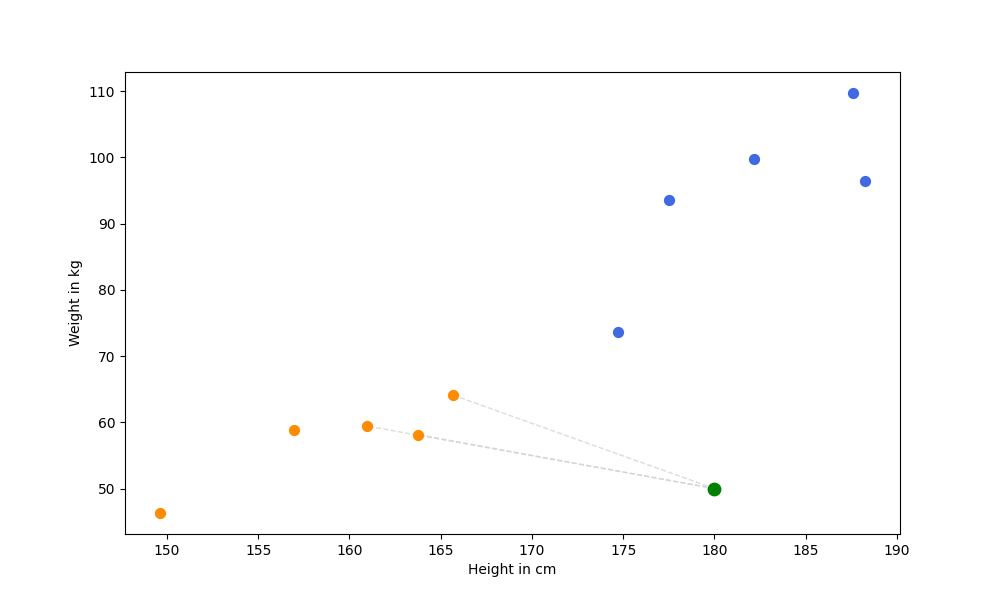
\includegraphics[width=1\linewidth]{Images/kNN/k-NN.png}
    \caption{grapfical depiction of k-NN algorithm}
    \label{fig:my_example}
\end{figure}

\textcolor{red}{\citep{yang2023outlier} for further information}


%After applying the global k-NN, the outlier scores are visualized by the bubble-size
%of the corresponding instance. The color indicates the label, whereas anomalies are red. It can
%be seen, that k-NN cannot detect the anomalies close to the clusters well and assign small
%scores \citep[p.8+9]{goldstein2016comparative}




\subsection{Minimum Covariance Determinant}
Statistical methods work differently then the methods discussed before. 
The methods making assumptions about the distribution of the data and  estimate population parameters, like mean and covariance.
Resulting in statistical inference, the method can predict with a percentage of how likely it is, that the analysed datapoint is an outlier.
In multivariate dataset, the covariance is an important parameter, because it describes the shape of the data in p-dimensional space.
Therefore using the mahalanobis distance, which incorporates the covariance, can be benefitial.
Naivy, by estimating the mean and covariance matrix and the resulting mahalanobis distance, you could define the $n$ largest distances as ourliers.


But the results of this procedure would be distorted by the masking effect.
Because the sample mean and covariance matrix are themselves sensitive to extreme values, a single outlier can pull the mean toward itself and inflate the covariance, essentially "masking" its own presence and leading to false negatives in outlier detection.
The MCD, proposed in 1984 by \citet{rousseeuw1984least} and later in 1985 theoretically justified in \citet{rousseeuw1985multivariate}, wasproposed as a solution to estimate robust estimators. 
Outliers bias non-robust estimators like the mean, by pullig it towards their direction.


This chapter is organized as follows: First I will explain the goal and the construction of MCD.


\subsection*{Theoretical Foundation}
The goal of MCD is to find a subset $H$ of $h$ \todo{which onw is right? h or n?} observations in a given dataset, with the minimal determinant.
As seen in Fig. the MCD draws the smallest possible ellipsoid, compared to classical methods \todo{which methods?}
When the smallest possible elipsoid is found, a robust distance, like the mahalanobis distance, is used to determine the distances between the subset mean (center) to the specific instance.
Intuitively,  as seen in figure, the goal of MCD is to draw an elipsoid around a subset of the data with the highest local density and not around the complete datatset, which will include outlier. 
Eliminating the masking effect of possible outliers.


%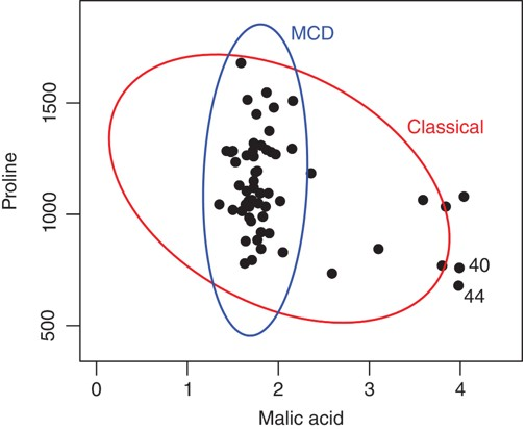
\includegraphics[width=\linewidth]{Images/MCD.pdf}


The MCD has a very high breakdown point.
The breakdown point describes the percentage of abitrary large instances that can be added without the estimator breaks down.
MCD will stay consistens even if 50\% arbirary datapoints are added to the dataset, thats the so called majority rule.
It does this by ignoring the instances outside the subset.
If the abitrary instances get above 50\%, MCD will prioritize those instances and not the subset anymore.
If the outlier ratio does exceed 50\% those cant be named outliers anymore, because they reach the status of inliers, because they are the mayority class. 


MCD is affine equvariant, that means, that the estimators stay consistent if affine transformations are undertaken.
Affine transformations are changes to the data, that does not change the geometric structure of the data.
In data preprocessing are affine transformation often used.
Rescaling data is an affine transformation, but the MCD estimators stay the same, instead of k-NN or deep learning models, that need to be normalized \citet{hubert2018minimum}.
  


\section*{FAST-MCD}
A disadvantage of the original algorithm is that it is computationally complex and for bigger dataset get impossible to estimate.
To find the matrix with the smallest determinant, you have to calculate all possible $\binom{n}{h}$ subsets.  
Therefore a more efficient algorithm, called FAST-MCD, was published in 1999 by \citet{rousseeuw1999fast} which includes concentration steps (C-Steps).
The FAST-MCD estimation is as follows:  

\begin{enumerate}
    \item Determine the number observations $h$ by applying $h = \frac{n+p+1}{2}$
    \item carry out two concentration steps
    \item for the 10 results with lowest $det(S3)$: carry out C-steps until convergence
    \item report the mean and covariance matrix with the lowest $det(S)$
\end{enumerate}
 
Instead it takes many initial choices of Subsets and are applying the concentrantion steps to each until convergence and keept the solution with the lowest determinant.
The C-Step algorithm is as follows:

\begin{enumerate}
    \item Initialize by drawing a random number $p+1$ subsamples $J$ and calculate the sample mean and the sample covariance matrix. If the resulting $det(S0)=0$ then add another random observation until $det(S0)>0$.
    \item If $det(S1)=/0$ compute the mahalanobis distances for all $n$
    \item To compute $H2$ sort the distances of (2) from smallest to biggest
    \item Select the $h$ smallest distances and compute the mean and coverance matrix
    \item Repeat until convergence
\end{enumerate}
\citep[p.214]{rousseeuw1999fast}


\subsection*{Implementation}
As above mentioned, I will calculate just two concentration steps with all initial subsets.
After that I will select the ten results with the smallest determinants.
I will do this selective iteration, because the distinction between robust and nonrobust solutions aleady becomes visible after two or three steps.  
\todo{add:rousseeuw, Driessen (1999)p.216 pp, nested extensions and explain why the algorithm is like this}
If one can be sure, that the dataset contains less then 25\% of outliers, you can choose $h=0.75n$ wich is a good compromise between breakdown value and statistical efficiency.
If the dataset contains many observations (e.g. n > 600), then you can create


\section*{Hyperparameter}
The MCD main hyperparameter is the number of observations in the subset $h$.
The range of $h$ is defined by: 


\begin{equation}
    \frac{n+p+1}{2} \le h \le n. 
\end{equation}


The lower boundary includes a minimum of 50\% of the data and additionaly the number of dimensions $p+1$.
If $p > h$ the resulting determinant of covariance matrix will be 0, hence the covariance matrix can't be inverted and the mahalanobis distances cant be estimated.
\citet{hubert2018minimum} recommends at least five observations per dimension to avaid excessiv noise. 

There is a trade-off relationship between the breakdown value and statistical efficiency.
The higher the robustness is chosen, the less efficient the estimators get. 
If the dataset does not contain more than 25\% of outliers, than it is suitable to choose $h  0.75n$. \citep[p.217]{rousseeuw1999fast}
The newly calculated estimator is less robust, but more efficient then before. 

The resulting $\hat{\mu}_{\text{MCD}}$ is the mean vector of the remaining subset $h$ which is used to calculate the mahalanobis distances.
The Mahalanobis Distance serves as a sophisticated metric for measuring the distance between a data point and the mean of a multidimensional distribution by including the covariance. 
It is defined as follows:


\begin{equation}
    D_M(\mathbf{x}, \mathbf{\mu}) = \sqrt{ (\mathbf{x} - \mathbf{\mu})^T \mathbf{\Sigma}^{-1} (\mathbf{x} - \mathbf{\mu}) }
    \label{eq:mahalanobis}
\end{equation}


Unlike the Euclidean distance, which treats all variables independently, the Mahalanobis Distance accounts for the correlations between dimensions by incorporating the inverse of the covariance matrix. 
This approach effectively standardizes the data, making the metric scale-invariant and allowing it to identify outliers that might appear normal when looking at single variables but are anomalous when viewed in combination.
In a statistical context, if a dataset follows a multivariate normal distribution, the squared Mahalanobis distance follows a Chi-squared distribution. 
This relationship allows researchers to perform parametric tests to flag outliers at a specific significance level. 


To detect outliers, the procedure includes an statisticall hypothesis test \todo{right? discordancy test}.
Testing if the observed datapoint comes from the same multivariante normal distribution as the rest of the data.
To calculate the test statistics, the mahalanobis distance needs to be transformed so it follows a $\chi^2$ distirbution.
The mahalanobis distances is transformed as follows:

\begin{equation}
    RD_i^2 = (\mathbf{x}_i - \hat{\mu}_{\text{MCD}})^T \hat{\Sigma}_{\text{MCD}}^{-1} (\mathbf{x}_i - \hat{\mu}_{\text{MCD}})
    \label{eq:robust_mahalanobis}
\end{equation}

If the mahalanobis distance of the suppodes outlier is greater than the critical $\chi^2$, the probability (p-value) wether this is an inlier is $1- \alpha$.
By increasing $\alpha$, I will increase the size of the elipsoid and an possible outlier has to be further away fromt the $\hat{\mu}_{\text{MCD}}$.
In this case the results will be more certain, but will restrict datapoint to be considered as outliers.


In my thesis I will implement a fixed threshold approach.
To ensure comparability, I will implement approach as described in the other two methods, which is to set the threshold to the outlier ratio.
Therefore, the MCD will rank the distances of datapoints to the MCD mean and the furthest $n\%$ will be defined as outliers.
The hypothesis approach does have an advantage in scenarios, where the outlier ratio is not known.
The detecting is adjusting accourdingly to the unknown outlier ratio.
Nevertheless, the outlier ratio in my experiments is known 


\section*{Variants of MCD}
Even recently reaseach has een done for new extension for MCD.
Because FAST-MCD begins by drawing random subsets, multiple runs of FastMCD on the same dataset may yield different results (a problem often mitigated by fixing the random seed in implementations). 
Furthermore, it requires drawing many initial subsets to ensure at least one is free of outliers, which can be computationally intensive. 
To circumvent both of these problems, the Deterministic MCD (DetMCD) algorithm was developed. \citep[p.621 pp.]{hubert2012deterministic}
DetMCD provides a deterministic approach to robust location and scatter. 
It uses the same iterative steps as FastMCD but avoids starting with random subsets, ensuring consistency. 
Unlike its predecessor, DetMCD is permutation invariant, meaning its result is independent of the order of observations in the dataset. 
Moreover, DetMCD typically runs even faster than FastMCD and is less sensitive to data contamination (outliers).


Briefly, MCD is defined by it high breakdownpoint, which ensures with even a very high outlier ratio a consistent estimation.
MCD does not need normalizations because it is adffine equivariant. 
This eleminates problems with normalization and ensures reliability even if scales are changed.
MCD mitigates the masking problem, making it a supplementary to the statistical hypothesis testing.
Lastly, the statistical approach of MCD making the results transparent and quantifiable, by assigning a probability to every datapoint.


On the opposite, even FAST-MCD is computationally complex and limited by the site of the dataset making it not suitable for modern big data applications.
MCD assumes a gaussian normal distribution and looses performance in dataset with different distributions.
MCD suffers from the Curse of Dimensionality, because it requires more instances than variables. 
The estimation is impossible if this requirement is not met.
FAST-MCD in peticular is a stochastic approach, which means, that two runs can estimate different results.
For solving this problem, there a variance of MCD that to solve it. \citep[p.5]{smiti2020critical}


I chose MCD as a benchmark because of its simplicity and statistical approach compared to the machine-leanring approach of the other methods.
It provides for the given dataset an answer wether the dataset justifies a complex algorithm like InterCont, or if a traditional statsistical method is enough. 
Moreover the affine equivariant charakteristic of MCD provides a second benchmark.
By comparing it to methods, that are not affine equivariant, I expect draw conclusions about the way InterCont learns the underlying geometry of the data \todo{achtung mit dieser aussage}